The goal in lab 1 was to implement the ALU of our processor. Our ALU supports 4
different modes:
\begin{enumerate}
    \item Addition
    \item AND
    \item NOT
    \item Compare
\end{enumerate}
To implement the addition mode we first made a full adder component and then
connected 8 of them together using a for generate block, creating a 8 bit ripple
carry adder. We did not do the optional carry lookahead adder.

We then used the adder to make a comparator, the comparator takes the two inputs
and subtracts one from the other. To do the subtraction we NOT the input and set
\textbf{CIN} = 1, this calculates the 2's complement of that number. The 
comparator then checks if the result is zero, if it is \textbf{EQ} = 1, else 
\textbf{EQ} = 0. The \textbf{NEQ} signal is just the opposite of \textbf{EQ}.

The AND operation was implemented using the built in AND between
STD\_LOGIC\_VECTORs. The NOT operation was a bit different, as it only uses one
of the ALUs inputs. It to was implemented using the built in NOT operation in
VHDL.

To combine all these components into one ALU we used a with select statement,
selecting the output from one of our components using the \textbf{operation}
input value. Finally, after the correct result had been chosen we checked if it
was zero to set the \textbf{isOutZero} output.

One of the assignments was to draw the block diagram of the full adder, by using
a half adder. That block diagram is included on the following page.
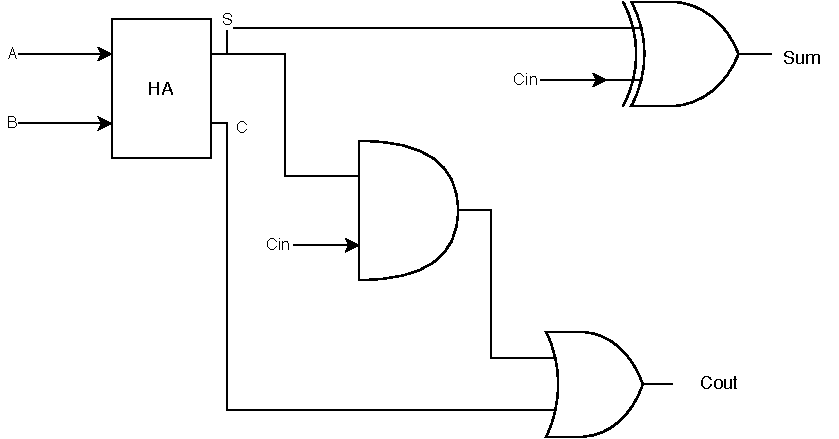
\includepdf{FullAdder.pdf}
